\chapter{Casos de Uso, Ejemplos y Resultados}\label{chapter:implementation}

En este último capítulo se intentará analizar desde todos los puntos de vistas
posible la propuesta de solución y su implementación concreta. Dicho análisis se
realizará con la intención de obtener una serie de resultados cuantitativos
basados en la experimentación para comprobar la valides de la propuesta realizada
como respuesta de los objetivos planteados. A lo largo de capítulo, el autor se
compromete a ser riguroso con la experimentación y sus resultados, además de aportar
una visión crítica y objetiva al interpretar dichos resultados.

Con cada uno de los experimentos realizados tiene como objetivo cuestionar la idoneidad
del sistema como respuesta de algún objetivo concreto de la investigación. Apoyadose en
los objetivos que se plantearon al inicio de la investigación, los cuales ya fueron
descritos en el capítulo introductorio, se formularon una serie de preguntas sobre las
cuales se diseñaron los distintos experimentos. De ser correcto el diseño de los
experimentos entonces en sus resultados se encontrarán las respuestas a las preguntas
planteadas y de ser dichas preguntas las adecuadas al final del capítulo el lector podrá
tener su propia opinión sobre el idoneidad de la propuesta de solución.

A lo largo del presente capítulo se espera que el lector pueda contar con las respuestas
de las siguientes preguntas. Primero, ?`qué tan expresiva es la herramienta?, ?`cuales son los
casos de uso de la misma?, ?`esta es más expresiva que resto de herramienta descriptiva que existen
en el estado del arte contemporáneo?. Segundo, ?`qué tan efectiva es la herramienta en el
proceso de generación de muestras?, ?`el sistema mantiene la coherencia entre las descripciones
y las muestras generadas?. Y por uúltimo, ?`qué tan eficiente es la herramienta?.

Para dar respuesta a esta última pregunta es necesario definir cuales son las características
que transformarían a la propuesta realizada en una solución eficiente para los objetivos
planteados. Por lo anterior, y haciendo referencia a lo ya mencionado en varias ocasiones,
se definen eficiencia para los objetivos propuestos con otras tres preguntas: 1) ?`qué tan
efectivas son las heurísticas implementadas para que el proceso generativo sea lo más lineal
posible, alejándose de las filosofías ``prueba y error''?, 2) ?`qué tan eficiente en tiempo es el
procesos de generación de muestras? 3) ?`es mejor utilizar el sistema propuesto para describir el
espacio de búsqueda y genera muestras de dicha descripción, que implementar de forma imperativa
un generador de dicho espacio con las herramientas nativas del lenguaje?.

A continuación se enumeraran los procesos de mayor complejidad algorítmica implementados.
Dicha información es muy importante para analizar los distintos experimentos y sus resultadas
que se mostrarán a lo largo del capítulo, pues con este conocimiento el lector podrá valorar
mejor el desempeño de la herramienta y la idoneidad de las implementaciones:
\begin{itemize}

      \item Generación de tensores: Para la construcción de los tensores los únicos datos iniciales
            que se tienen son la dimensiones de este y su tipo. Por dicha razón la implementación de este
            procesos describe una iteración recursiva donde se van generando cada uno de los indices internos
            y con cada indice generado se crea su muestra respectiva.
      \item Segmentación del dominio de los enteros por la operación distinto (!=) con una lista de valores: Cuando el usuario describe
            una desigualdad entre el dominio del los enteros y una lista de valores para poder crear los
            segmentos correctos es necesario ordenar dicha lista. Por tanto dicho procesos es más costoso que
            revisar si un elemento no pertenece a la lista de valores señalados.
      \item Restricciones secuenciales que referencian a subsecciones del propio espacio: Restricciones de
            este tipo implican que para cada uno de los indices del espacio es necesario construir una segmento nuevo
            con los elementos señalados, lo cual es un tanto más costoso que una simple comprobación sobre la misma
            referencia
      \item Resoluciones de restricciones de caja negra que no aportan datos al procesos de inferencia: Como ya
            se señalo anteriormente, dichos procesos únicamente pueden ser resueltos con el mecanismo de “prueba y error”,
            por lo que su costo temporal depende de las dimensiones del espacio y la probabilidad de seleccionar un elemento
            factible según la distribución en cuestión
      \item Resolución de dimensiones dinámicas: Este es sin duda el procesos más crítico para el mecanismo generador,
            pues en este casos no se pueden realizar cálculos previos en fase de compilación pues no se conocen los detalles
            del espacio. A su favor, los espacios descritos con estos mecanismo no presenta una descripción simple en el resto
            de los mecanismo descriptivos.
\end{itemize}

El resto del capítulo se divide en dos secciones. En la primera se describirán uno a uno los
experimentos realizados y se reportarán sus respectivos resultados. En la siguiente y última,
el autor realizará un análisis crítico y objetivo de los resultados obtenidos en los experimentos
y sobre el sistema en general.

\section*{Experimentos, Descripción y Resultandos}

Para intentar mostrar todas las características y particularidades de la propuesta el autor diseñó
cuatro experimentos con los que espera dar respuesta a las preguntas anteriormente planteadas. El
autor considerá que los experimentos diseñados le permitirá al lector tener una noción del
comportamiento del sistema en la mayoría de sus casos de uso, además de reflejar la gran variedad de
casos de uso a los que dicho sistema puede dar respuesta.

\subsection*{Ejemplos, Generación y Consistencia}

El primero de los experimento consiste precisamente en la explotación del {\bf DSL} para evidenciar la
amplia gama de dominios que este puede describir y generar. El desarrollo de este experimento
formó parte activa del proceso de desarrollo, el cual siguió un patrón orientado a pruebas ({\bf Test
            Driver Design}). Dicho patrón plantea que el desarrollo se realice única y exclusivamente con el
objetivo de vencer una prueba definida previamente. Como el objetivo final del sistema es la
generación de muestras aleatorias, dichas pruebas fueron implementadas con una visión estadística,
buscando el 100\% de casos positivos en la mayoría de dichas pruebas.

El código de los ejemplos de caso de uso se puede consultar en las secciones iniciales del presente
documento. En dicha sección se ordenan dichos ejemplos en orden ascendente a la complejidad de los
mismo. A continuación se enumerarán cada uno de dichos ejemplos, verbalizando el espacio de búsqueda
que se intenta describir en cada casos, puntualizando las distintas consideraciones tomadas a la hora
de implementar sus respectivas pruebas y realizando en cada caso las debidas comparaciones con el
estado del arte en términos expresivos:

1) {\bf Búsqueda acotada por las características previamente conocidas de la mejor recta que ajuste los
            datos}. En este casos el espacio de búsqueda se describe como una clase simple donde las restricciones
no contienen dependencias contextuales ni mayor complejidad. Para validar que la herramienta es
coherente con la descripción aportada por cada una de las muestras generadas se comprueba que dicha
muestra pertenece a la clase descrita y que los atributos que representan la pendiente y el intercepto
de la recta se encuentran dentro de los limites descritos para cada uno.

Todas las restricciones descritas en este casos hacen referencia a los limites del espacio exceptuando
la operación de desigualdad (!=), describiendo la existencia de un elemento incorrecto en el interior del
dominio inicial. En este casos todas las herramientas descriptivas basada en clases como {\bf AutoGOAL} y
      {\bf AutoSklearn} puede detectar dicho elemento dentro del cuerpo de la función {\it \_\_init\_\_} y lanzar el error
respectivo. {\bf Optuna}, por otro lado, al tener una sintaxis imperativa puede optar por varias opciones:
1) la ``prueba y error'', 2) la definición de dos dominios disjuntos seleccionables a partir de
una variable aleatoria que distribuya como una bernoulli. Dicha última opción, sería el único enfoque
mediante el cual aquellas herramientas que describen su espacio de búsqueda mediante funciones de
distribución pudieran modelar dicha separación del dominio inicial.


2) {\bf Búsqueda de un punto óptimo en el interior del un dataset con una estructura particular}, todos los
puntos se encuentra contenidos por las rectas {\it x = y + 10} y {\it x = y - 10}. En este caso el espacio de búsqueda
si es sensible al contexto, pues la variable x depende del valor de la variable y. Como se puede ver en la
implementación del ejemplo, la descripción es una clase simple con la sintaxis antes descrita para definir
dependencias contextuales. Para validar la consistencia de las muestras generadas en la respectiva prueba se
comprueba que el punto generado se encuentre en el interior de la franja descrita por dichas rectas empleando
las debidas inecuaciones.

Como ya se señalo en el capítulo número dos la única herramienta del estado del arte contemporáneo capaz de
describir dependencias contextuales es la biblioteca {\bf Optuna}, que efectivamente puede describir este espacio
realizando una generación en orden topológico, implementada de forma imperativa. El enfoque descriptivo basado en clases
puede utilizar la filosofía de ``prueba y error'' para solo analizar las instancias que cumplan con la condiciones
descritas. En el casos de las bibliotecas de optimización que se apoyan en los diccionarios y las funciones de
distribución, no tiene forma de expresar dicha relación.

3) {\bf Optimización paramétrica}, donde la descripción del espacio de búsqueda del conjunto de parámetros de la clase
      {\bf LogisticRegresion} de {\bf Sklearn} refleje lo descrito en su documentación oficial en cuanto a la semántica de dichos
parámetros. La gran mayoría de las clases y modelos aportados por {\bf Sklearn} y otras bibliotecas suelen definir varios
parámetros condicionales y dependientes del contexto. En el casos particular de la clase seleccionada, la semántica
de los parámetros ``intercept_scaling'' y ``random_state'' depende del valor específico del parámetro ``solver''. Al ser
un espacio condicional en este casos la implementación de las respectivas pruebas consiste en determinar a cual de
los posibles casos pertenece la muestra en cuestión para luego comprobar sus distintos atributos.

Como a pesar de que el ejemplo muestra un espacio condicional, este sigue siendo un casos de dependencias contextuales
por lo que la comparación expresiva es similar a la del caso anterior. En este caso únicamente señalar que debido a que
las herramientas descriptivas basadas en clases, como es el caso de {\bf AutoGOAL} o de {\bf AutoSklearn}, no cuentan con estructuras
de flujo para describir dependencias condicionales, entonces para valores dependientes de este estilo siempre se genera
una muestra de sus dominio más amplio independientemente de que se use la misma o no.

4) {\bf Búsqueda de los plazos óptimos para programar dos tareas rutinarias que nunca deben coincidir}. En este caso se hace
referencia al espacio de dos números naturales primos relativos entre ellos. Dicha relación no puede ser expresada
combinando los distintos operadores definidos en la gramática de restricciones, por lo que se define una función de
``caja negra'' para describir dicha restricción. En este caso, para cada muestra la prueba implementada revisa que no
exista ningún número natura que divida a ambos atributos. Igual que en los dos casos anteriores, en este ejemplo existen
dependencias contextuales, por lo que las herramientas expresivas en el estado del arte son limitadas.

5)y 6) {\bf Modelación de grafos}. Como se puede ver en ambos ejemplos el {\bf DSL} es capaz de modelar el espacio de búsqueda donde
la estructura del mismo es un grafos. El sistema propuesto puede modelar grafos utilizando los dos diseños más comunes de
estas estructuras, las matrices de adyacencia y los grafos orientados a objetos. La teoría de grafos es una de las
herramientas más potentes para resolver problemas de búsqueda.

Aunque el objetivo de dichos dos ejemplos es evidenciar la capacidad de la herramienta para describir los espacio con forma
de grafo, los dos patrones de diseño planteados para dichas estructuras utilizan herramientas muy distintas del sistema. Las
matrices de adyacencias se modelan mediante la representación de dependencias circulares internas. Para comprobar las muestras
generada por dicho espacio se comprueba iterativamente si la matriz generada es simétrica y si sus dimensiones corresponden a
la respectiva cantidad de nodos generados. Por otro lado, el modelo orientado a objetos hace uso de la integración de la
herramienta con la biblioteca {\bf typing}. Dicho espacio por su descripción es propenso a generar errores del tipo {\bf RecursionError},
pues según su descripción existen elementos en el espacio con dimensiones infinitas. Por lo anterior, en la prueba realizada a
dicho espacio se comprueba que mínimo la mitad de las muestras sean finitas y que cada una de ellas cumplen con las
restricciones estructurales definidas.

La descripción de estos espacios es extremadamente complicado en el resto de las herramientas analizadas. La opción más común
para describir espacios similares es la representación de listas de adyacencia. Aunque en principio las herramientas basadas
en clases podrían describir los grafos orientados a objetos, ellas no presentan ninguna sintaxis para describir la opcionalidad
de los subespacios internos de la clase en cuestión. La representación más parecida a las propuestas presentadas serían son las que se pudieran
definir con la biblioteca {\bf Optuna}, pero dicha implementaciones serían muy similares a los generadores de muestras implementables
con las herramientas nativas del lenguaje.

7) {\bf Modelación del clásico problema de ``la mochila'' como problema de búsqueda}. Dicho espacio de búsqueda se describe como una
jerarquía de clases donde de forma independiente se definen distintos conceptos como: los elementos que pueden formar parte de
la mochila, la estructura de la mochila y la estructura de la solución para un problema dado. En este ejemplo se evidencia que la
herramienta no solo generar muestras para los parámetros iniciales de los constructores de las distintas clases, como es el caso de
      {\bf AutoGOAL}, sino que además es capaz de realizar llamadas a métodos de las instancias generadas empleando parámetros aleatorios. La
prueba implementada para dicho espacio consisten en dos procesos de comprobación estadística: 1) generación de múltiples posibles
problemas y comprobación de la correcta estructura de las distintas muestras, 2) generación de múltiples soluciones para cada uno
de los distintos problemas generados y comprobación de que cada una de ellas es una  soluciones factible del problema en cuestión.

Muchas de las herramientas del estado del arte podrían aporta una descripción del espacio de búsqueda de soluciones para un problema
dado, incluyendo en la mayoría de los casos múltiples elementos no factibles dentro de las descripciones pues el espacio de
soluciones factibles es un espacio sensible al contexto. Pero solo {\bf Optuna} podría describir a la vez el espacio de los posibles
problemas con sus posibles soluciones, aunque nuevamente dicha descripción no estaría muy alejada de la implementación que se podría
lograr con las herramientas nativas del lenguaje.

8) {\bf Modelación del clásico problema de búsqueda “el mapa de colores” y su espacio de soluciones}. Al igual que en el caso anterior,
en esta ocasión se muestra que la herramienta propuesta es capaz de describir el espacio de todas las instancias del problema en
cuestión junto al conjunto de posibles soluciones para cada una de las instancias. En trabajos futuros a las dos componente descritas
en el presente trabajo se le debería integrar un tercer componente capaz de modificar las distintas distribuciones aleatorias. Por
lo antes expuesto no se le desarrollo al sistema ninguna estrategia de búsqueda para la generación de espacios combinatorios. Por
todo lo anterior el DSL no puede generar el espacio de soluciones factibles del problema planteado. En este caso el autor propone
una descripción lo más detallada posible, donde ante cada selección se compute el conjunto de colores adyacentes para que el mecanismo
generador intente elegir en cada caso un color correcto. Dicho conjunto de colores debe transformarse en el conjunto vació en caso de
ser el conjunto total de colores. Aunque al realizar dicho cambio ya se conoce que la instancia resultante no será un elemento factible,
en el futuro con la integración de un sistema optimizador todas las instancias serán importantes para determinar las distribuciones
más eficientes.

De forma similar al caso anterior, el proceso de prueba se divide en dos momento, la generación de problemas y la generación de
soluciones. Para cada uno de los problemas se comprueba su correcta estructura y la pertenecia de cada uno de sus atributivos a sus
respectivos dominios. Por otro lado, el análisis de las soluciones es un poco más dinámico pues para cada una de las selecciones
realizadas se comprobará el dominio dinámico que computó la herramienta para realizar dicha selección.

Al igual que en ocasiones anteriores, la optimización sobre dicho espacio combinatorio solo podría ser descrito por la biblioteca
      {\bf Optina}, realizando una análisis similar al propuesto para cada uno de los indices que fuera a generar.

9) {\bf Descripción del espacio de búsqueda de un pequeño problema de AutoML con dependencias contextuales}. En este casos se plantea la
búsqueda de un modelo de aprendizaje automatizado semisupervisado, donde en el espacio de búsqueda descrito se evidencia los
problemas clásicos del {\bf AutoML}: la selección de modelos y la optimización paramétrica. En dicho ejemplo se muestra como se puede
describir dicho espacio de búsqueda con una jerarquía de clases y como se relacionan las mismas planteando una dependencia contextual
en los niveles superiores de la jerarquía (la clase {\bf AutoMLUnsupervidedExample}), restricción que afecta al dominio de un elemento
particular que tiene en común cada uno de los modelos que participa en el procesos de selección de modelos. Dicho ejemplo es un
resultado más de la integración del {\bf DSL} con la biblioteca {\bf typing}

El procesos de prueba para este casos de uso se limita a la comprobación de la estructura de las muestras generadas. Cada uno de
los modelos debe pertenecer al tipo base correcto independientemente a la
selección del modelo final. La restricción planteada para el número de clusters y la cantidad de categorías debe cumplirse tambien.
A nivel descriptivo, todas las herramientas que soluciona el problema de la selección de modelos y la optimización paramétrica
cuenta con herramientas para describir dicho espacio de búsqueda. Aunque en la mayoría de los cosos la restricción planteada sería
implementada de una forma más imperativa, generando un único valor y compartiendo el mismo para las dos instancias seleccionadas.

En resume, el primer experimento consiste en la implementación de una lista de ejemplos utilizando el {\bf DSL} propuesto para luego generar
un número representativo de muestras y comprobar que efectivamente dichas muestras pertenecen al espacio descrito. El código de las
pruebas se puede consultar en el repositorio de {\bf GitHub} de la propuesta de solución. En dicho repositorio se puede consultar además los
resultados de dichas pruebas, las cuales se ejecutan con cada modificación del código mediante el empleo de los {\bf GitHub's Actions}.
El autor confirma que cada una de las pruebas tuvo un resultado correcto y que todos los ejemplos presentados son se pueden describir y
generar con el sistema propuesto.

\subsection*{Casos Simple. Comparación con las herramientas nativas}



El segundo experimento consiste en cronometrar del desempeño del mecanismo generativo del {\bf DSL} propuesto para los casos más simples y
básicos. Luego se comparan los resultados del {\bf DSL} con los resultados de un experimento similar realizado a los generadores implementados
con las herramientas nativas del sistema. Aunque el objetivo de este experimento es comprobar la rápidez de generación del sistema,
también se mostrará el costo temporal del sistema como un todo, uniendo el procesos de interpretación con la generación de muestras,
como evidencia de todo lo explicado anteriormente sobre la descomposición del {\bf DSL} en dos tiempos, compilación y ejecución.

Como ya se ha comentado anteriormente, dentro del sistema existen tres procesos generativos básicos, dos aleatorios y un tercero
constructivos. En dicho segundo experimento se comparará la rápidez del {\bf DSL} para generar un entero, seleccionar un texto, crear una
clase o crear una lista con las respectivas implementaciones análogas utilizando las herramientas nativas del lenguaje. A continuación
se enumeran y detallan cada una de las comparaciones
\begin{enumerate}
      \item Generación de un número entero mediante: 1) el sistema como un todo, 2) la componente generativa, 3) generador basado en la función {\it uniform} de la
            biblioteca {\it random}. Se generaron 10000 muestras y cada una de ellas dentro de subconjunto [-100000, 100000] de los enteros.
            Cada una de las generaciones se cronometraron utilizando la biblioteca {\it time} de {\bf Python}.
      \item Selección de un elemento contenido dentro de una lista de opciones mediante: 1) el sistema como un todo, 2) la componente generativa,
            3) generador basado en la función {\it uniform} de la biblioteca {\it random}. Se generaron 10000 muestras y cada una de ellas se eligió entre
            todos los textos contenidos en una lista que guarda cada uno de los números naturales del 0 al 1000 escritos de forma textual. Cada una de las
            generaciones se cronometraron utilizando la biblioteca {\it time} de {\bf Python}
      \item Generación de una lista de número entero mediante: 1) el sistema como un todo, 2) la componente generativa, 3) un mecanismo generador
            implementado mediante la sintaxis de compresión de listas de {\bf Python} y generador basado en la función {\it uniform} de la biblioteca {\it random},
            4) un mecanismo generador implementado mediante la sintaxis de compresión de listas de {\bf Python} y el mecanismo generador del
                  {\bf DSL} para generar números enteros . Se generaron 10000 muestras y cada una de las listas generadas tienen longitud 1000 elementos.
            Cada elemento en las listas están definidos dentro de subconjunto de los enteros [-10000, 10000]. Cada una de las generaciones se cronometraron utilizando la
            biblioteca {\it time} de {\bf Python}.
      \item Generación de una clase cuyo constructor espera dos número entero mediante: 1) el sistema como un todo, 2) la componente generativa,
            3) un mecanismo generativo implementado mediante el constructor de dicha clase y generador basado en la función {\it uniform} de la biblioteca {\it random}, 4) un
            mecanismo generativo implementado mediante el constructor de dicha clase y el mecanismo generador del {\bf DSL} para generar números enteros.
            Se generaron 1000 muestras y en cada una de ellas los distintos parámetros son generados están definidos dentro del subconjunto de los
            enteros [-10000, 10000]. Cada una de las generaciones se cronometraron utilizando la biblioteca {\it time} de {\bf Python}.
\end{enumerate}

\begin{figure}[!ht]
      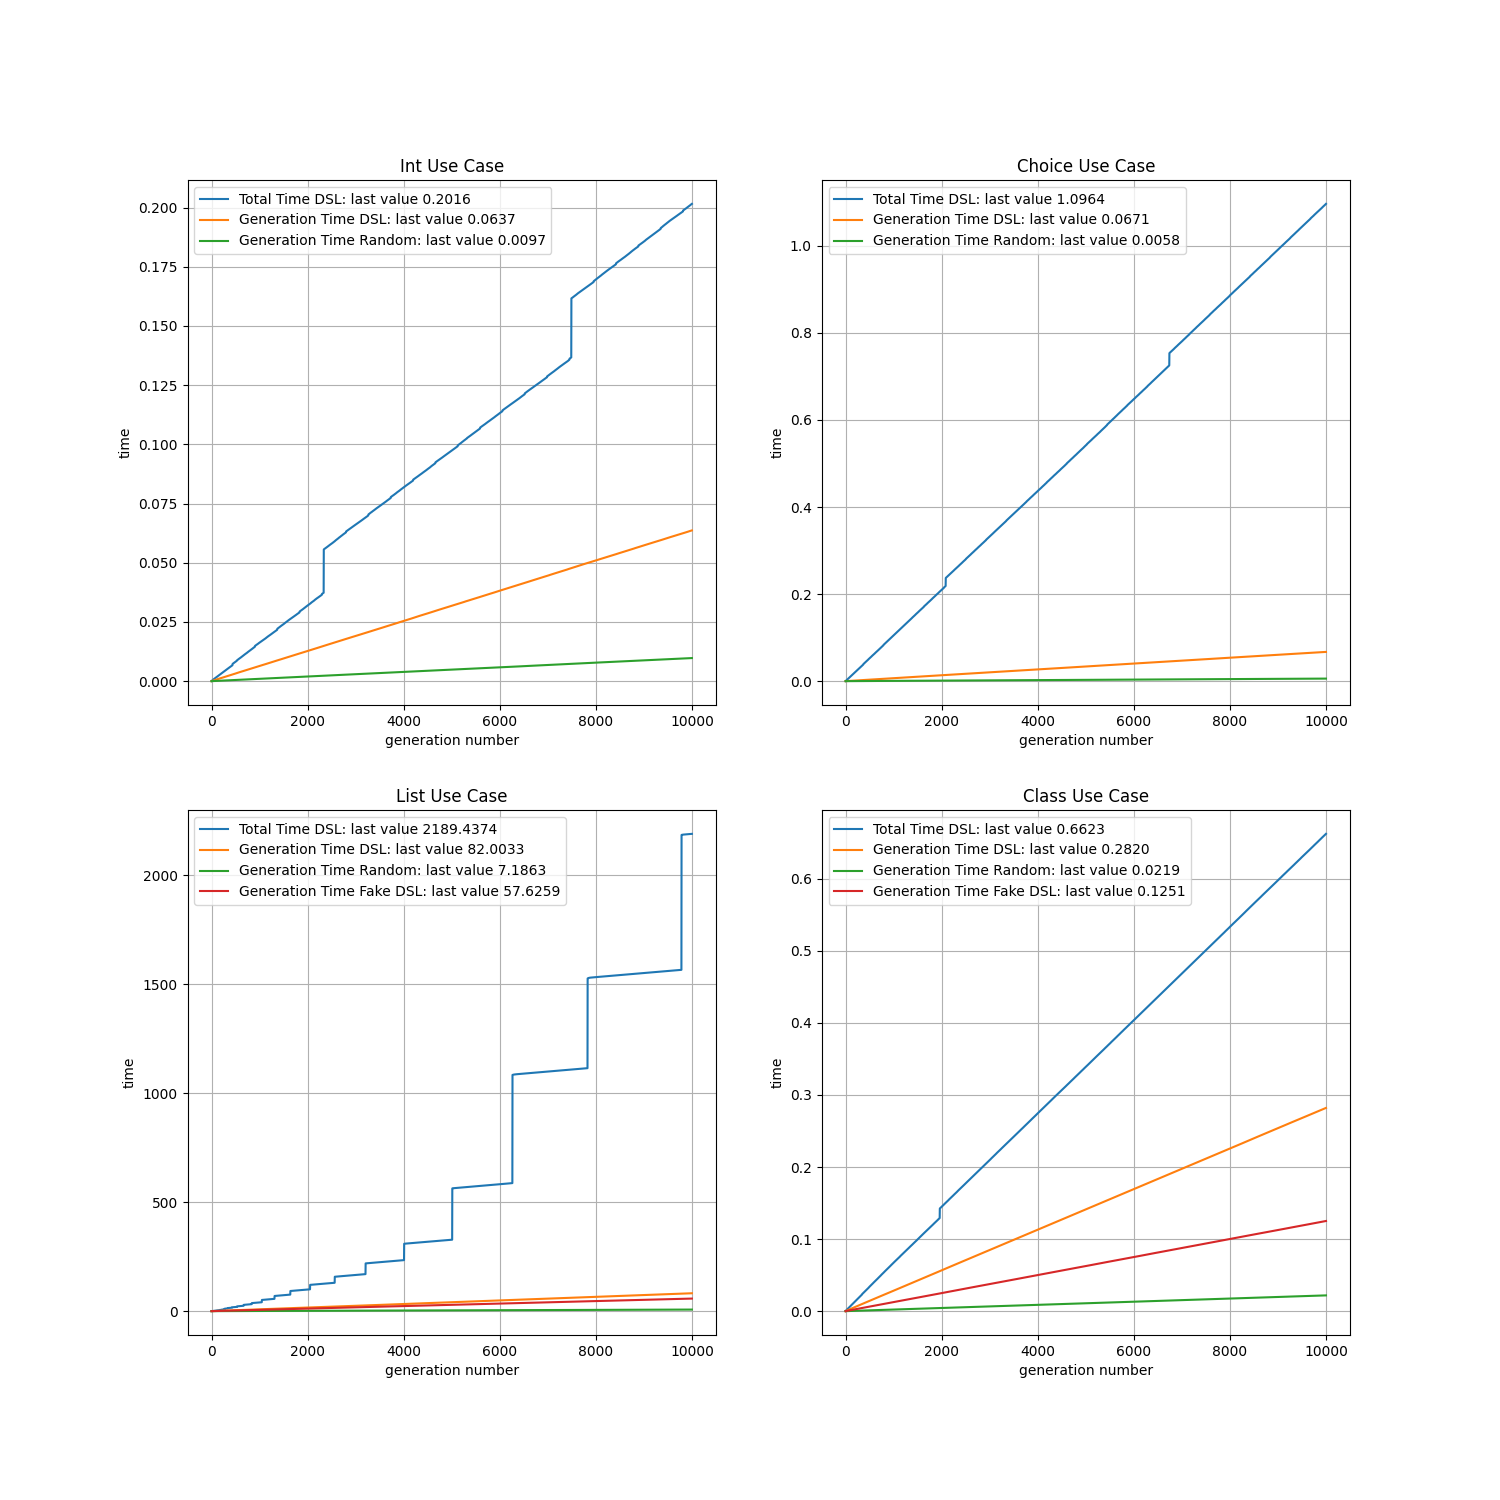
\includegraphics[width=\linewidth]{Graphics/exp2.png}
      \caption{Resultados del Segundo Experimento}
      \label{fig:exp_2}
\end{figure}

\subsection*{Procesos más costosos, conjuntos y matrices simétricas}

El tercer experimento consisten en la medición de la eficiencia en cuanto a tiempo y exploración
del espacio de los ejemplos más simples en los que aparecen los procesos más costosos antes
mencionados. Dichos ejemplos son: 1) la generación de conjuntos, donde se tiene una operación de
diferencia que segmenta los dominios enteros mediante lista y la referencia a subsecciones del
espacio subyacente, y 2) la generación de matrices simétricas, donde se evidencia el costo de
la generación de tensores de múltiples dimensiones. Para estos casos se realizaron 3 experimentos:
\begin{enumerate}
      \item Generación de 1000 conjuntos, donde para cada iteración {\bf i} se generó un conjunto de tamaño {\bf i}
            tal que los elementos en su interior se encuentran definido en el espacio de los naturales entre
                  [0, 1000]. Dicho experimento se realizó un total de 100 veces y los resultados finales reportado
            responde a la media de los resultados obtenidos.
      \item Generación de 1000 conjuntos, donde para cada iteración {\bf i} se generó un conjunto de tamaño {\bf i}
            tal que los elementos en su interior se encuentra definido en el espacio de los naturales entre
                  [0, {\bf i} + 1 ]. Dicho experimento se realizó un total de 100 veces y los resultados finales reportado
            responde a la media de los resultados obtenidos.
      \item Generación de 100 matrices simétricas, donde para cada iteración {\bf i} se generó una matriz de
            tamaño ({\bf i} + 1, {\bf i} + 1) tal que los elementos en su interior se encuentran definido en el espacio de los
            naturales entre [0, 1000]. Dicho experimento se realizó un total de 100 veces y los resultados
            finales reportado responde a la media de los resultados obtenidos.
\end{enumerate}


\begin{figure}[!ht]
      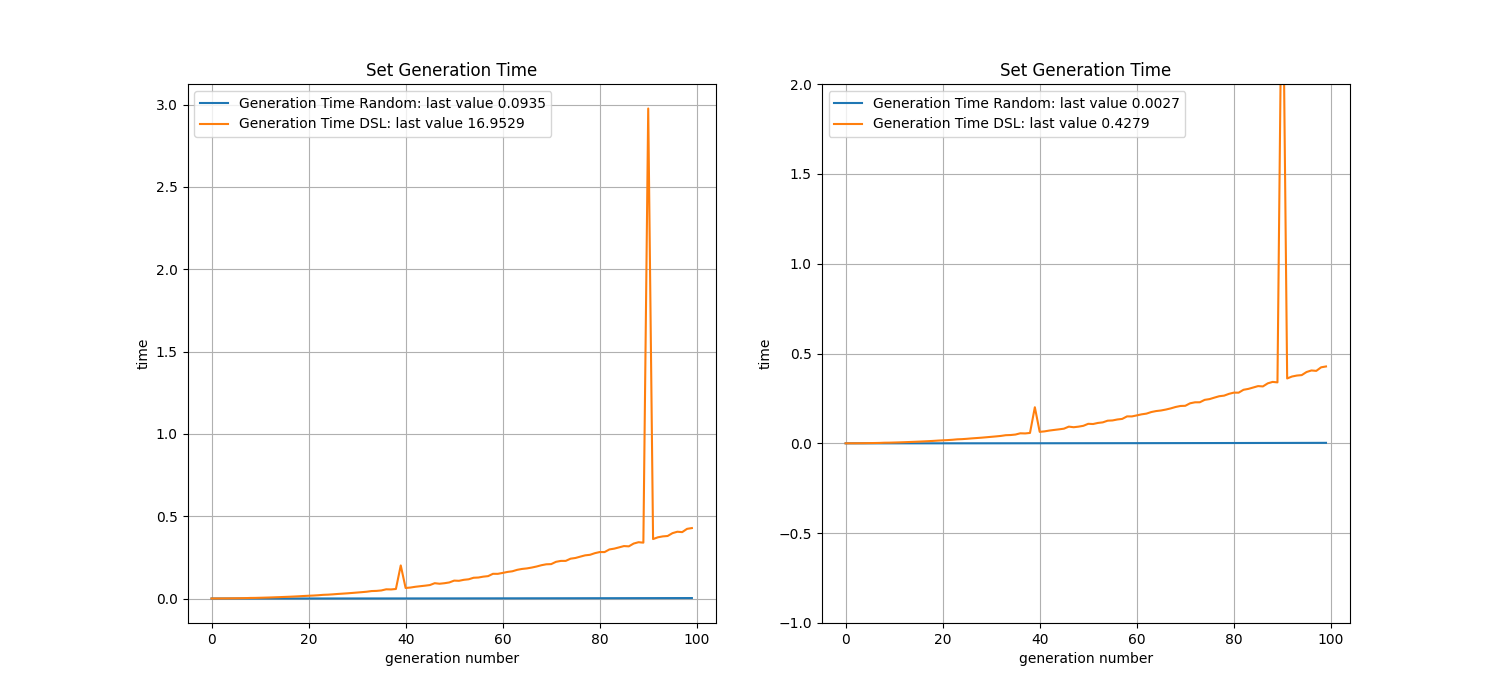
\includegraphics[width=\linewidth]{Graphics/exp4.png}
      \caption{Resultados de los experimentos con matrices}
      \label{fig:exp_4}
\end{figure}

En cada uno de los experimentos se midierón el tiempo de generación y, para el caso de los experimentos
con conjuntos, el número de error a la hora de elegir un nuevo elemento para el conjunto, donde un error
es elegir un elemento que ya pertenezca al conjunto. Las generaciones fueron realizadas por: 1) el
mecanismo generador del sistema y 2) generador basado en la función {\it uniform} de la biblioteca {\it random}.
En las dos siguentes gráficas se muestran los resultados obtenidos.

\begin{figure}[H]
      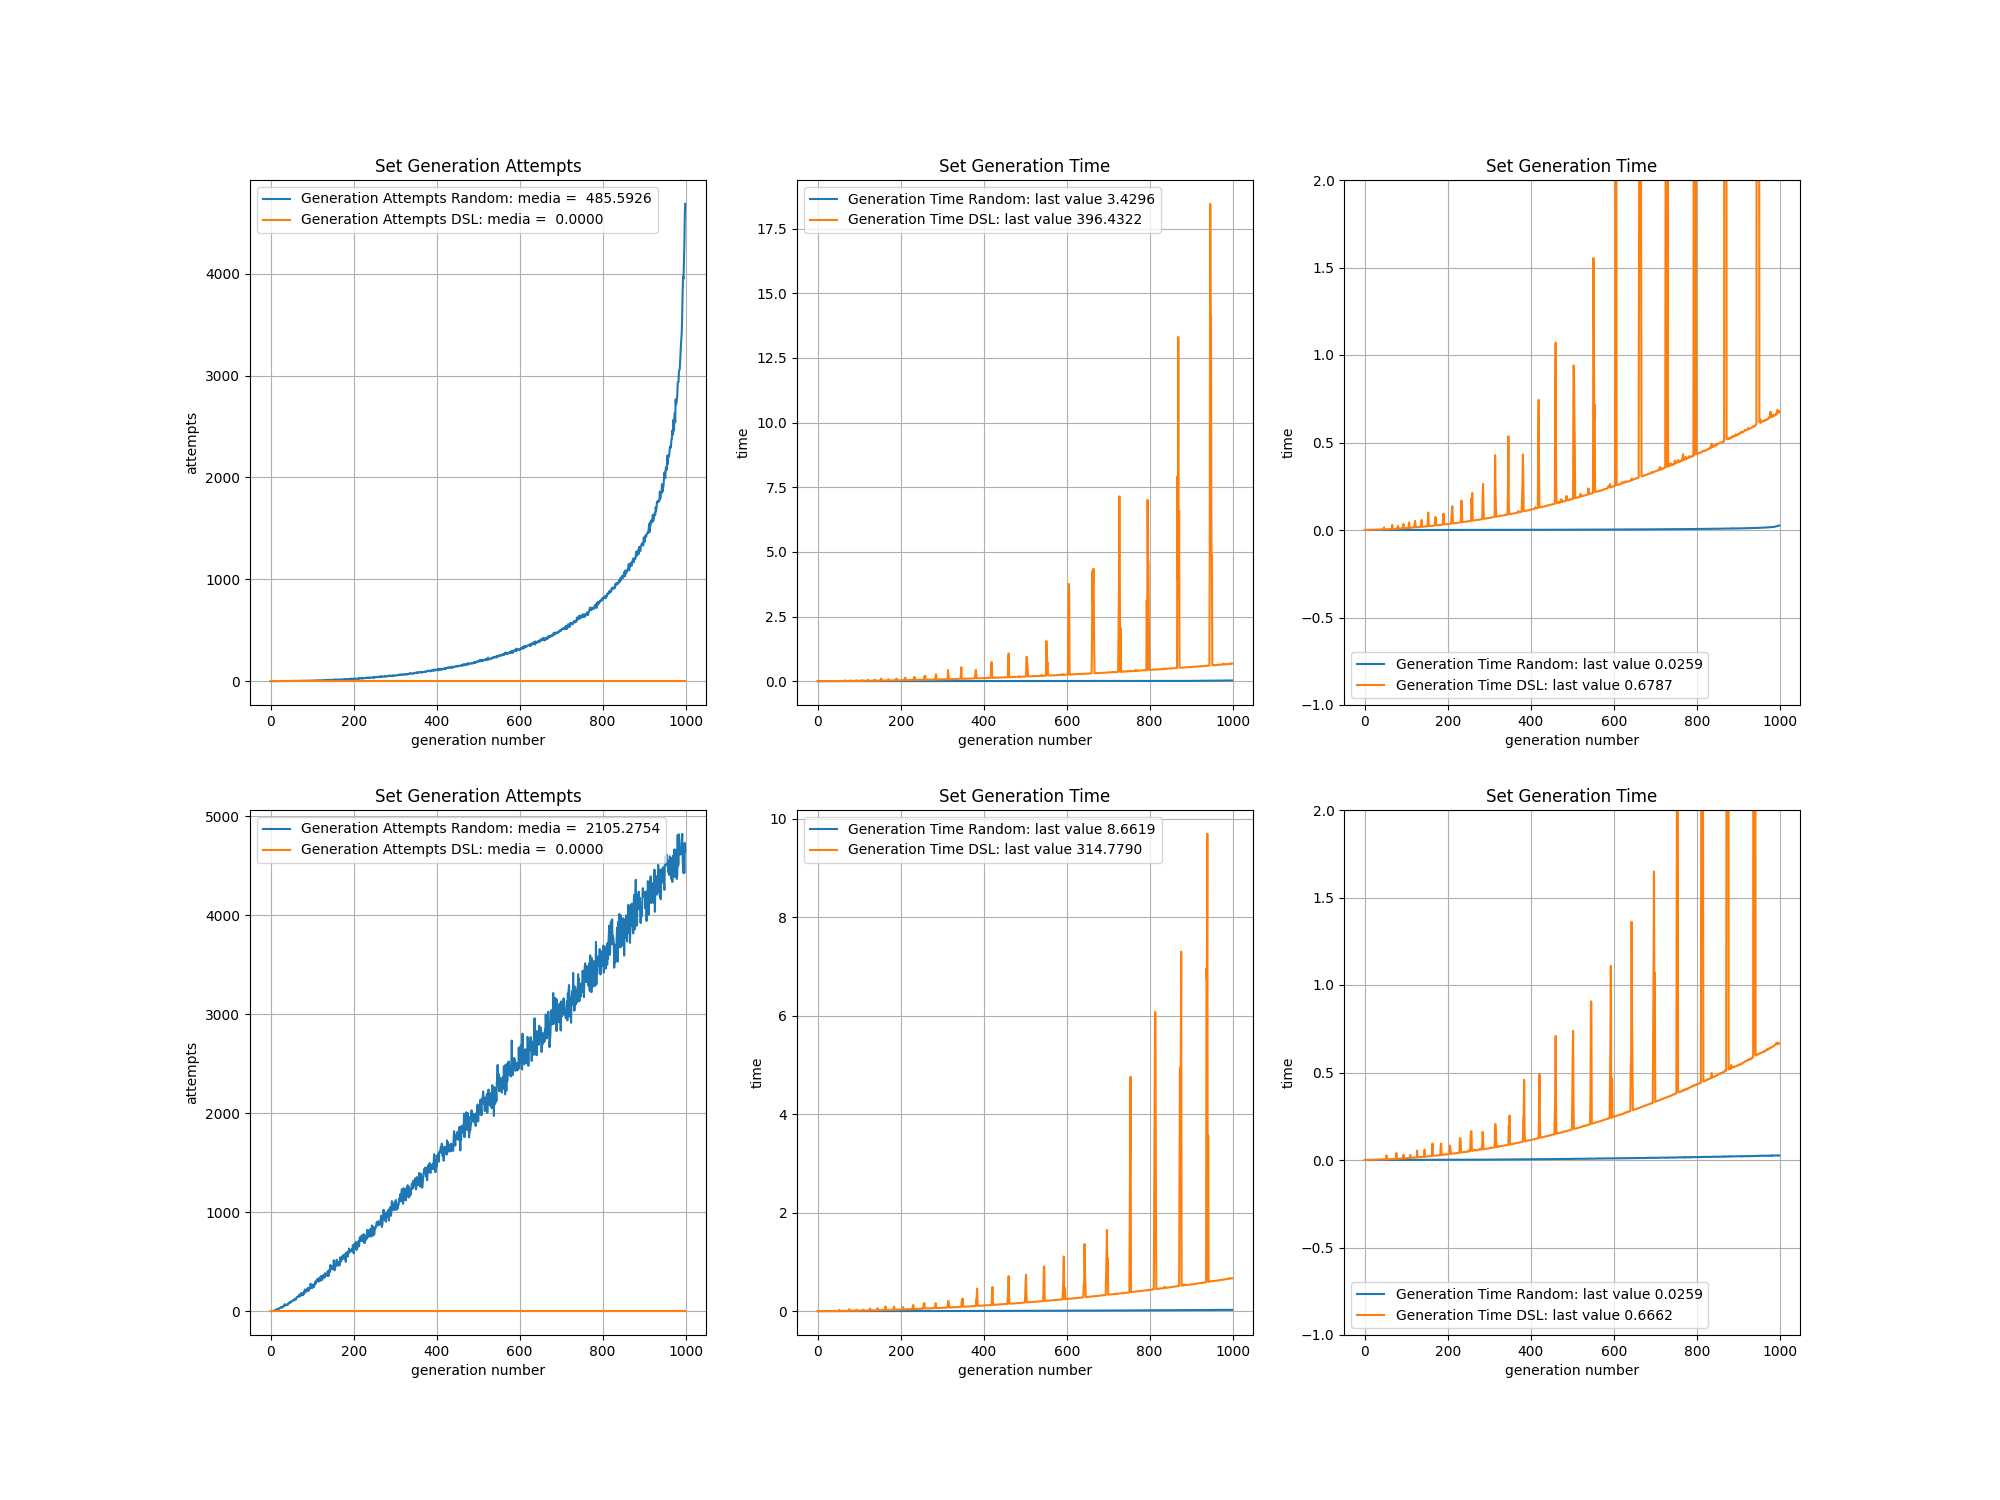
\includegraphics[width=\linewidth]{Graphics/exp3.png}
      \caption{Resultados de los experimentos con conjuntos}
      \label{fig:exp_3}
\end{figure}



\subsection*{Heurísticas para restricciones de caja negra}

Los casos de funciones de “caja negra”, como ya se ha explicado con anterioridad, es en ocasiones la
funcionalidad más estocástica del sistema, pues para aquellas restricciones que se definen una dependencia
con los elementos del espacio subyacente el único procesos generativo posible es la “prueba y error”.
Además como ya se ha señalado en capítulos anteriores, existe una diferencia determinante cuando se le
aplica dichas restricciones a espacios compuestos como las listas o las clases y cuando se le aplica a
espacios simples como los números. Cuando una espacio sencillo como los números presenta una restricción
de “caja negra” que no se puede incluir en el proceso de inferencia de dominios, el sistema plantea una
heurísticas de búsqueda muy simple. Aprender de cada error cometido modificando el dominio de generación.
Dicha heurísticas no es posible en el casos de los espacios estructurales pues dichos espacios son
combinatorios y descarta opciones no es trivial.

El cuarto experimento realizado intentó evidenciar el efecto de dicha heurísticas en la eficiencia temporal
y de exploración del mecanismo generativo ante casos de funciones de ``caja negra'' que no aportan información
al proceso de reducción de dominios. Dicho experimento esta compuesto por dos parte y en ambas se utilizará
la función {\bf IsEven} definida en capítulos anteriores.

El primero de los experimentos realizados consiste en la generación de 500000 números primos donde para cada
generación {\bf i} se definen el espacio de búsqueda en el subconjunto de los naturales [2, {\bf i} + 100]. Con este
experimento se busca encontrar el tamaño de dominio a partir del cual la heurísticas es determinante en el
costo temporal del proceso generativo. A dicho experimento se someterán 3 generadores:
\begin{enumerate}

      \item  El mecanismo generador del sistema planteado apoyado en la respectiva descripción del espacio
      \item  Un generador implementado mediante las herramientas nativas del lenguaje
      \item  Un generador implementado con las dos componentes principales del sistema generativo propuesto, el
            dominio y la función de distribución. En cada iteración el dominio se expande en vez
            de crearse uno nuevo. De esta forma el autor desea comprobar que tan determinante sería la persistencia del
            aprendizaje, funcionalidad que no se implementó en primera instancia por incompatibilidad con los casos de
            dominios dinámicos y dependencias contextuales.
\end{enumerate}

De este experimento se cronometró el tiempo de generación y se contabilizaron tanto el número de errores como la
cantidad de errores repetidos. Los resultados se muestran en las gráficas siguientes.

\begin{figure}[H]
      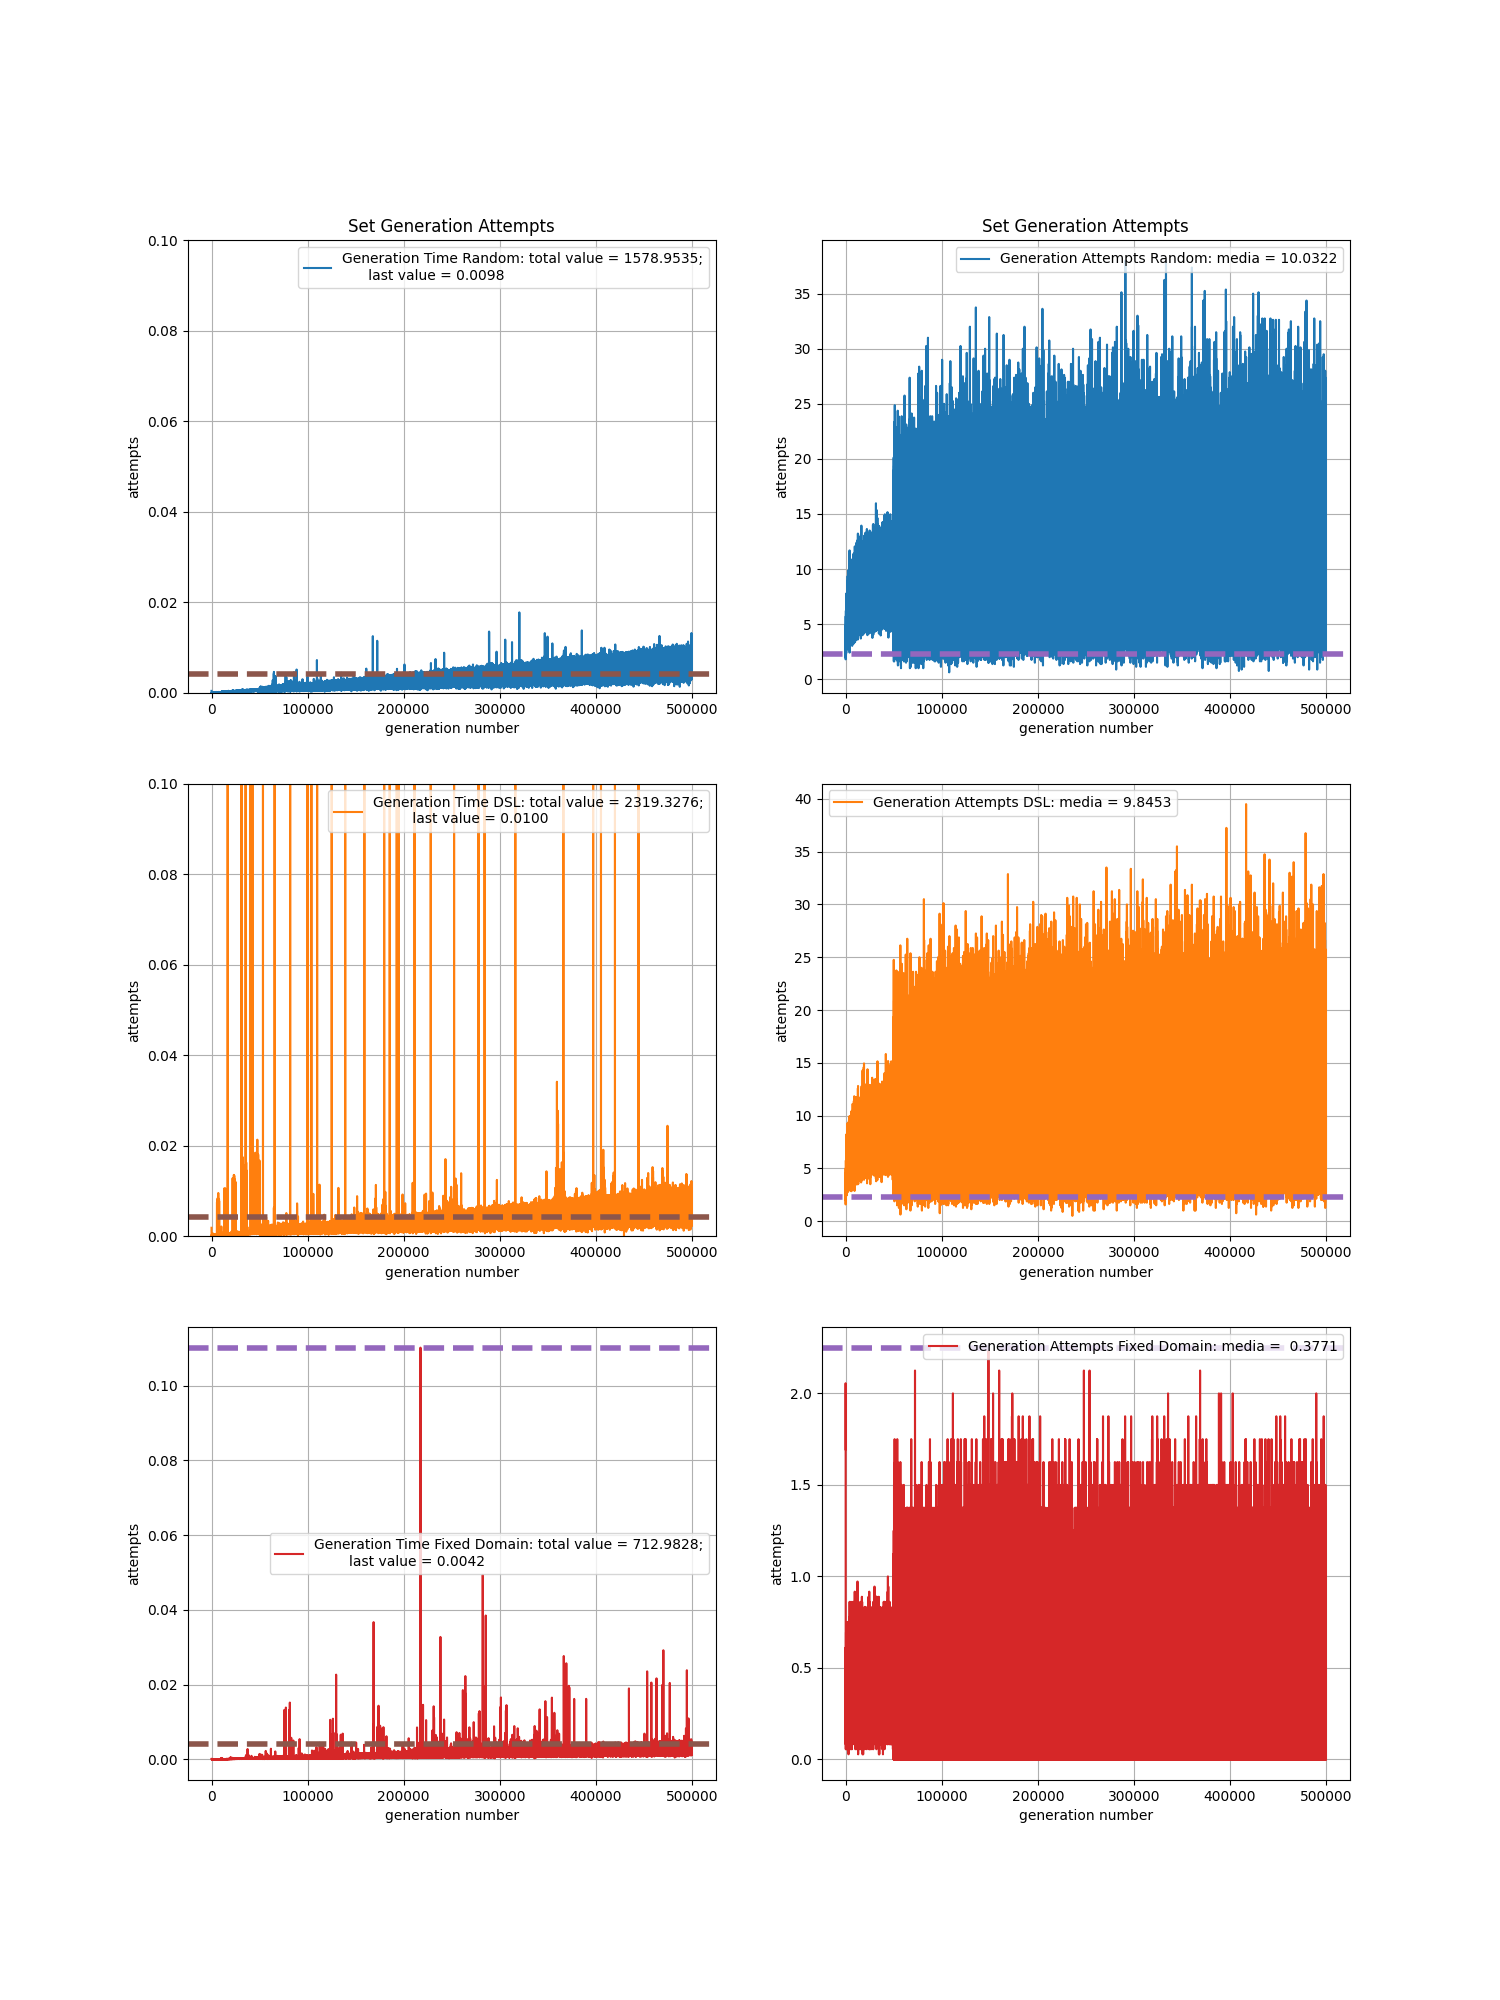
\includegraphics[width=\linewidth]{Graphics/exp5.png}
      \caption{Resultados de la primera fase del 4to experimento}
      \label{fig:exp_5}
\end{figure}

La segunda fase de este experimento número 4 es la generación de números primos con limites fijos. Dicho experimento
es un complemento a la pregunta planteada en el tercer generador de la fase anterior. ?`Qué tan determinante sería
la persistencia del aprendizaje obtenido en cada generación?. Para dicho experimento se generaron 500000 números primos
dentro del subconjunto [2, 250000 ] de los números naturales. En este casos se usarón los mismos 3 generadores de la
fase anterior solo que en este casos el tercero de ellos no se expande en cada iteración. De este experimento se cronometró
el tiempo de generación y se contabilizaron tanto el número de errores como la cantidad de errores repetidos. Los resultados
se muestra en las dos siguiente figuras

\begin{figure}[!ht]
      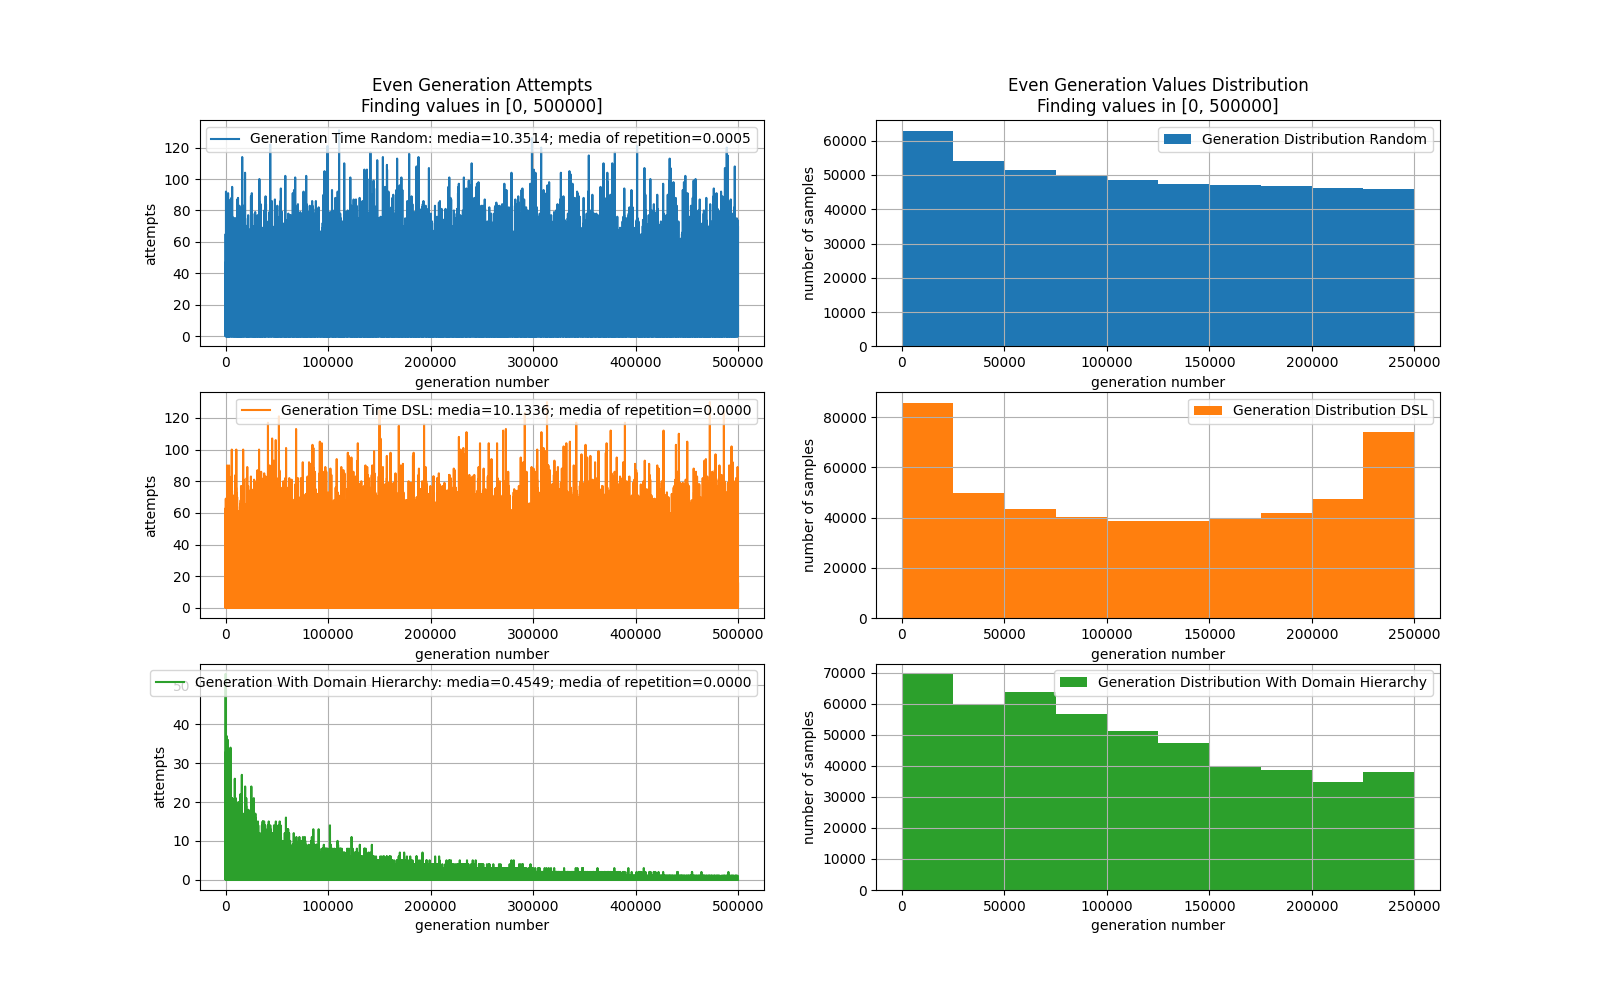
\includegraphics[width=\linewidth]{Graphics/exp7.png}
      \caption{Grafica de intentos y distribucion de muetras la segunda fase del 4to experimento}
      \label{fig:exp_7}
\end{figure}

\newpage

\begin{figure}[H]
      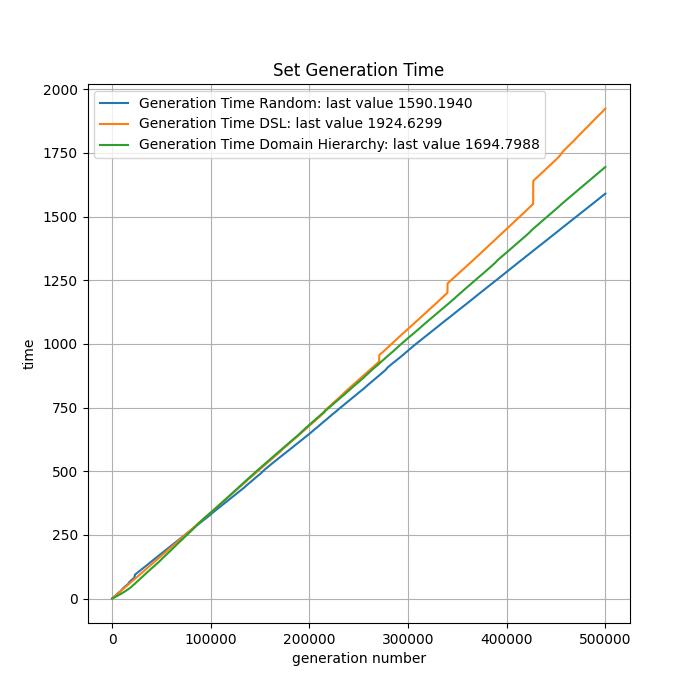
\includegraphics[width=\linewidth]{Graphics/exp6.png}
      \caption{Grafica temporal de la segunda fase del 4to experimento}
      \label{fig:exp_6}
\end{figure}

\subsection*{Discusión}

Analizando los resultados obtenidos en los experimentos anteriores se pueden realizar varias observaciones.
Primero, como ya se había comentado con anterioridad el mecanismo generador de forma generar no puede ser más
rápido que un generador implementado de forma imperativa con las herramientas nativas del lenguaje. En los
resultados obtenidos en los experimentos realizados con los casos básicos se evidencia que para todos ellos un generador
imperativo es mucho más rápido que el mecanismo generador. Independientemente a esto, se puede señalar que a
excepción de la generación de listas la diferencia entre los tiempos óptimos y los del sistema planteado no es
extrema, considerando además el número de generaciones realizadas.

Segundo, en el mismo experimento se evidencia además el gran acierto que supuso la comprensión de la herramienta
como dos componentes y la delimitación de los momentos de cada uno de ellos. Nótese la inmensa diferencia entre
los tiempos reportados por el mecanismo generativo por si solo y los obtenidos por el sistema como un todo. Tercero,
en contraste con los resultados obtenidos en los experimentos realizados para analizar al mecanismo generativo donde
dichos resultados requieren de una interpretación y un análisis para poder ratificar su valides, los resultados
obtenidos en durante los experimentos realizados con la componente descriptiva es una prueba irrefutable de que la
herramienta propuesta aumenta no solo el número de espacio de búsqueda descriptibles sino que además lo hace con
mucha mayor expresividad que las herramientas del estado del arte contemporáneo.

Luego, en el experimento realizados sobre los casos más críticos se pueden ver varios resultados que ponen en duda
que las ideas planteadas e implementadas sobre la reducción de dominios sean determinantes en la reducción de los
costos temporales del mecanismo de generación. Pues; como se muestra en los resultados de dichos experimentos,
en especial para los casos en los que se experimentó con el espacio de los conjuntos hasta las dimensiones exploradas,
independientemente del número de errores que comenta el mecanismo imperativo el costo temporal de la infraestructura del
sistema es mayor que el del mecanismo de “prueba y error” implementado de forma imperativa. Nótese, que en los resultados
de dicho experimento la linea temporal del mecanismo generador presenta una serie de picos temporales. Dichos picos se le
atribuyen al sistema de almacenamiento de cada uno de los espacios creado con su respectiva función de distribución,
dicho mecanismo fue implementado mediante una clase que sigue el patrón {\bf Singleton}. Por las característica de los experimentos
realizados, donde en cada iteración se crea un nuevo espacio, el diccionario interno de la clase antes mencionada pasa a ser
ineficiente múltiples veces si necesita expandir su tabla de hash y recolocando cada uno de los elementos. Dicho fenómeno no
debería ocurrir en situaciones normales, pues como ya se comentó anteriormente las descripciones y las generaciones no debería
ocupar el mismo espacio de ejecución.

Dicho mecanismo de almacenamiento fue implementado preparando al sistema para la futura incorporación de un mecanismo
optimizador. Al igual que el protocolo de reducción de dominios, aunque se demostrará que no es eficiente para la
generación de muestra en casos específico, es parte fundamental en la resolución de dependencias contextuales. Siendo ambos ejemplos
de procesos en principio necesarios que forman parte de la infraestructura del sistema para resolver distintos problemas
y que para ciertos casos pueden no ser favorables.

El experimento final, entre otras cosas, fue influenciado por la incertidumbre causada por el experimento precedente.
En el mismo se buscó describir desde múltiples puntos el mecanismo de reducción de dominios. Como se puede ver en la
colección de resultados de la primera fase de este cuarto experimento, independientemente
al aprendizaje de los espacios de búsqueda planteado en cada iteración el costo temporal del {\bf DSL} sigue siendo superior
al del generador imperativo. Además como en cada generación con la implementación actual del {\bf DSL} el aprendizaje se pierde,
entonces se puede ver que el número de intentos de generación son muy similares, con la única diferencia de que uno repite
valores erróneos y el {\bf DSL} no. Al igual que sucede en los experimentos anteriores, analizando los tiempos reportados y el problema
al que se le intenta dar solución los resultados no son del todo malos, las diferencias temporales podrían llegar a ser
despreciables.

En dicho primer pasos del experimento cuatro el autor incluyó un tercer generador para investigar cuan determinante sería
realizar una factorización del sistema para persistir el aprendizaje de generaciones anteriores. Nótese que la optimización
sería ampliamente efectiva, reduciendo casi a la mitad el tiempo de generación en comparación con los métodos nativos del
lenguaje. Además de por supuesto disminuir representativamente el número de errores de generación cometidos. Por dichas
razones, aunque ya existía evidencia para recomendar dicho desarrollo, como este experimento muestra un empleo inapropiado de
sistema, pues como se ha comentado anteriormente estos experimentos hace que la compilación y la generación ocupen el mismo
espacio.

Para medir el impacto real de dicha factorización en el sistema se realizó el segundo paso del experimento número 4. En la
primera fase el dominio que mantendría el aprendizaje se fue expandiendo en cada iteración, pero dicho caso no tendría lógica
en un escenario real pues si un domino se encuentra definido dentro de cierta segmentación es porque el resto de los valores
del espacio son no son factible. Realizar una expanción sería, en principio, agregar valores erróneos al domino. Por dicha razón
el segundo pasos determina unos limites fijos de búsqueda, un caso más real del caso de uso que se piensa factorizar. Como se
puede ver la gráfica en la que se muestra los tiempos reportados por dicho experimento mientras que el {\bf DSL} siempre es más lento
que el mecanismo imperativo, dicho sistema con la factorización planteada se acercaría mucho más a los tiempos reportados por
las herramientas nativas del lenguaje.

Aunque evidentemente la refactorización planteada mejoraría la eficiencia del sistema, de este último experimento aun se puede
comentar algunos detalles. Primero, el experimento se realizó delimitado por un parámetro {\bf n} donde {\bf n} es el número de generaciones
que se realizarán y dichas muestras se encontrarán definidas entre [0, {\bf n}/2]. Como se puede ver en la gráfica que muestra el
número de errores de generación se aprecia que aunque el dominio va aprendiendo de sus errores al final del experimento sigue
existiendo valores erróneos. Esto significa que una vez que se empieza a segmentar el dominio existe un punto en donde la
probabilidad de escoger un segmento totalmente valido para generar una muestra es mucho mayor que la de escoger un segmento
invalido, por lo que empiezan a aparecer generaciones que no aportan aprendizaje. El experimento muestra que 500000
generaciones no son suficientes para que el sistema explore un espacio de [0, 250000] de forma aleatoria.
Luego, nótese además la influencia de la refactorización en la distribución de las muestras. En el casos del {\bf DSL} planteado
por la presente investigación existe mayor densidad de muestras en los extremos del dominio, mientras que la distribución
de la factorizacón se muestra más uniforme. Por lo que en resumen, sería una muy buena idea incluir la modificación de los
dominios iniciales para los espacios simples.

Finalmente, el autor considera el resultado como un éxito tanto en términos descriptivos como generativos, independientemente
de que los resultados obtenidos por el mecanismo generador no eran los esperados. En general los tiempos obtenidos por el
mecanismo generador presenta una diferencia con respecto a los tiempos de los mecanismo imperativos implementados que podrían
considerarse despreciables considerando la expresividad del código final y la seguridad en la generación de muestras. Como se
mostró en el primer experimento realizado la gama de espacios descriptibles con la herramienta es representativamente grande y
variada, además de que las pruebas implementadas para garantizar la coherencia del sistema es una prueba bastante fiable para
confiar en que cualquier descripción implementada con la herramienta generar nuestras del espacio descrito.

La presente investigación surgió para, en parte, encontrar una solución para las limitaciones expresivas de {\bf AutoGOAL}. En este
sentido el autor opina que indudablemente la integración de la biblioteca con el {\bf DSL} planteado ampliaría el espacio de problemas
optimizables por {\bf AutoGOAL}. Pero el autor cree que dicha integración favorecería más a los problemas de búsqueda clásicos o la
transformación de problemas simples, que al problema principal de la herramienta (el {\bf AutoML}). En este sentido, existen pocos modelos
con restricciones tan fuertes como para que la dilatación del proceso de generación de muestras sea representativo frente a la
evaluación de la función objetivo, que supone el entrenamiento y evaluación de los distintos pipelines.